\subsection{U-Boot 启动软件}

系统启动程序基于官方 U-Boot v2026.07，参考清华 JIT 团队的uboot优化，并针对我们的 SoC 完成板级移植。上电后由 FPGA MIG 完成 DDR3 初始化与校准，处理器随后从 SPI Flash 启动；U-Boot 初始化直接映射窗口、Cache、串口与网络设备，确认并使用 128\,MiB SDRAM，将自身从 Flash 执行区重定位到 SDRAM，最终进入 \texttt{u-boot@LoongsonSoC\#} 命令行。

\subsubsection{板级适配}

主要适配内容包括：
\begin{itemize}
  \item LA32R 启动入口、重定位、Cache 初始化、计时器和 16550 串口；
  \item 128\,MiB SDRAM 容量识别与重定位、SPI Flash、非 PCI DC2114x Ethernet MAC 与板级设备树；
  \item 非一致 DMA 所需的 cached/uncached DMW 地址转换和 \texttt{dbar} 所有权屏障；
  \item Linux ELF 装载和跳转前的 Cache 清理、屏障与启动参数传递。
\end{itemize}

当前网络驱动使用 32 个 RX descriptor 与 4 个 TX descriptor，配置 full-duplex、store-and-forward 和发送阈值；RX packet buffer 使用 uncached 映射，避免每包重复 Cache sweep。TFTP 默认块大小为 1468\,B、窗口大小为 1。当前 SoC 没有 SD/MMC 控制器、引脚或设备树节点，因此启动路径不包含 SD 卡。

\subsubsection{TFTP 启动 Linux}
U-Boot 2026.07 已在 CPU 为 60\,MHz 的当前 SoC 上完成实际启动，并可通过串口进入命令行、通过 TFTP 加载 Linux 镜像。TFTP 加载速度高达 500 KB/s。

\begin{figure}[H]
  \centering
  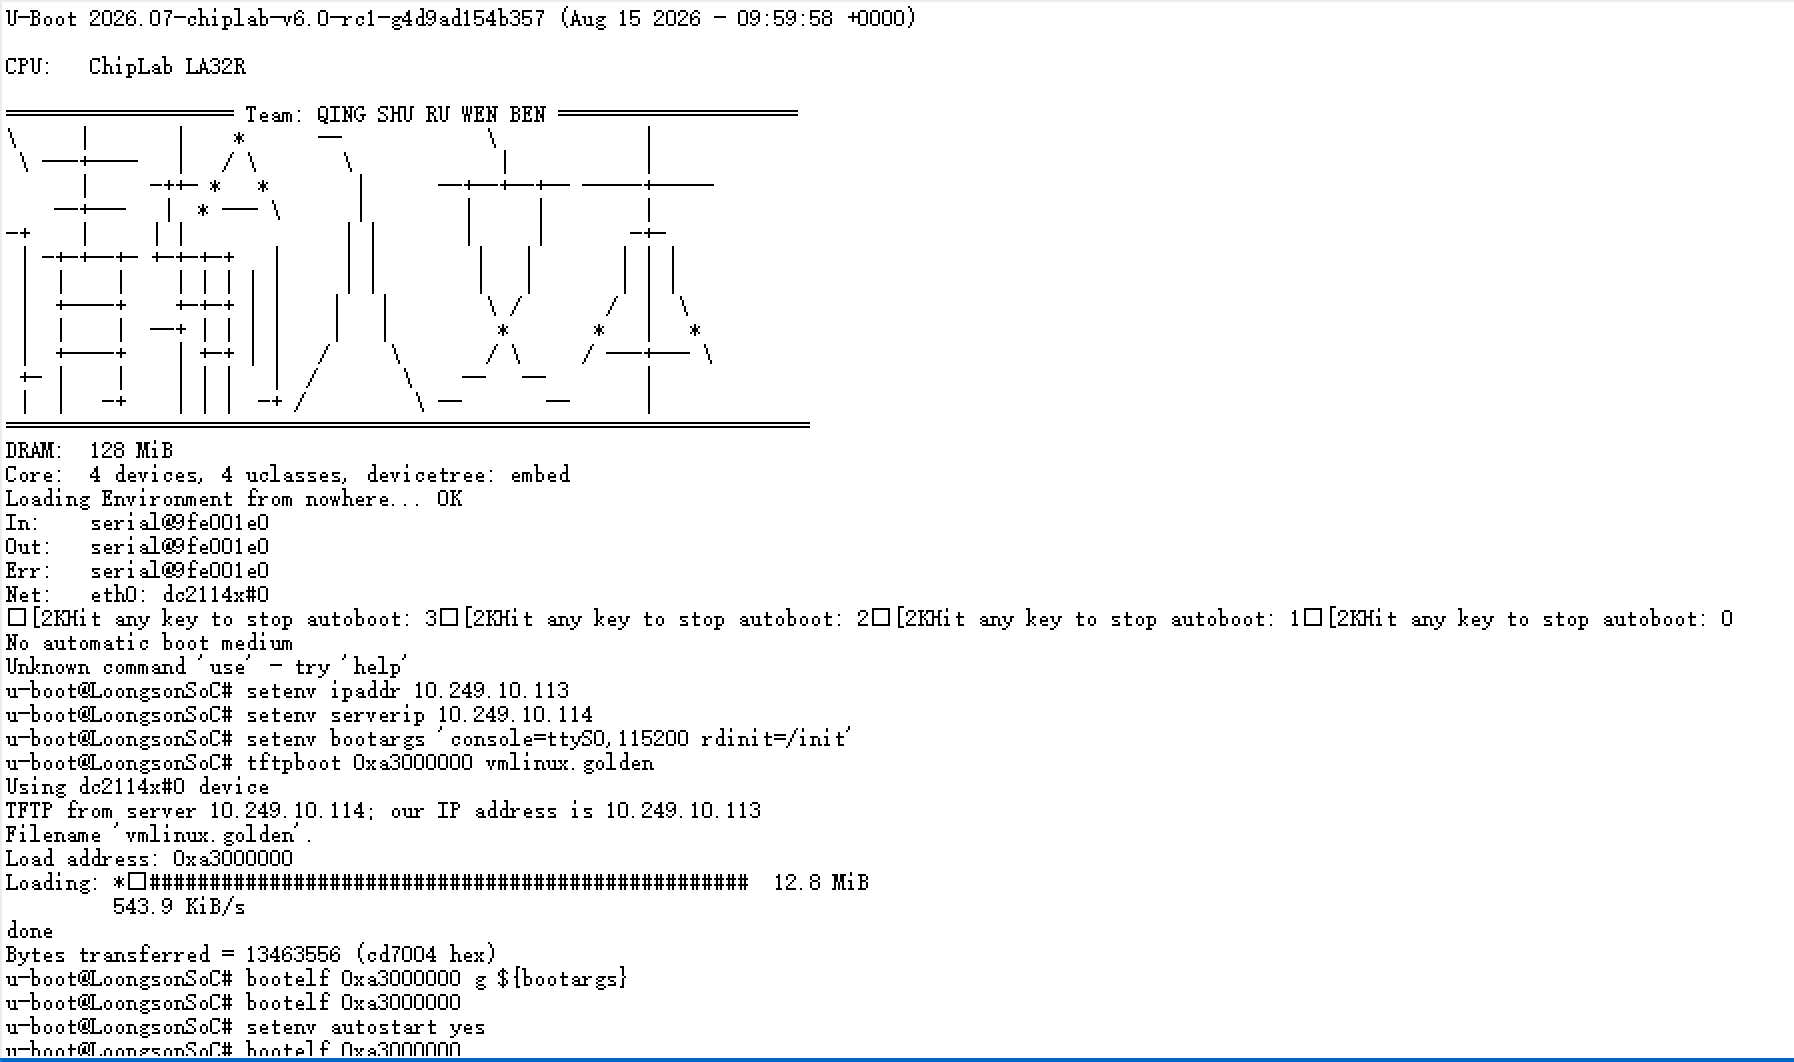
\includegraphics[width=0.95\textwidth]{figure/uboot.png}
  \caption{uboot启动linux}
  \label{fig:uboot}
\end{figure}
